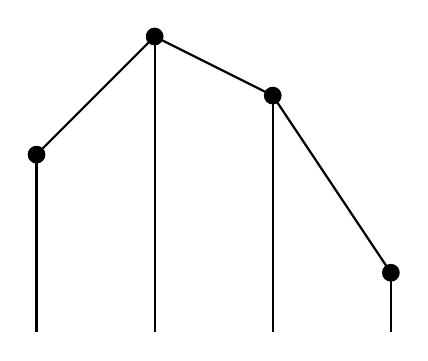
\begin{tikzpicture}[scale = 1.5]
    \def \valY{{2, 4, 3, 0.5}}

    \foreach \x in {0,...,3}{
        \pgfmathsetmacro\asInt{int(\valY[\x])}
        \pgfmathsetmacro\r{(\asInt+1)/2}
        \draw[thick, black, -](\x,0) -- (\x,\r);
        \draw[fill = black](\x,\r) circle (2pt);
        
        \pgfmathsetmacro\nextx{\x==3 ? \x : \x+1}
        \pgfmathsetmacro\nextAsInt{int(\valY[\nextx])}
        \pgfmathsetmacro\nextR{(\nextAsInt+1)/2}
        \draw[thick, black, -](\x,\r) -- (\nextx,\nextR);
    }
\end{tikzpicture}